\documentclass[12pt]{article}
\usepackage[utf8]{luainputenc}
\usepackage[danish,british]{babel}
\usepackage{listings}
\usepackage{hyperref}
\usepackage{xcolor}
\usepackage{graphicx}
\usepackage{float}

\DeclareGraphicsExtensions{.png}

\lstset{
	breaklines=true,
	basicstyle=\tiny,
	language=bash,
	keywordstyle=\color{blue},
	numbers=left
}

\title{Opgave 1}
\author{Christoffer Wadum Larsen}

\begin{document}
\maketitle

\section{Part 1}

\subsection{Q1}

\begin{lstlisting}
[chris@localhost opgave2]$ sudo chmod 755 S1.bash 
[chris@localhost opgave2]$ ./S1.bash 
Hello world Happy Birthday
[chris@localhost opgave2]$ 
\end{lstlisting}

\subsection{Q2}

These variables are local. When opening a new terminal they will be uninitialized.

\begin{lstlisting}
[chris@localhost opgave2]$ echo $VAR1

[chris@localhost opgave2]$ 
\end{lstlisting}

\subsection{Counting files}

\begin{lstlisting}
[chris@localhost opgave2]$ alias how_many_files="ls -1 | wc -l"
[chris@localhost opgave2]$ how_many_files
9
[chris@localhost opgave2]$ alias how_many_files='VAR4="`pwd` contains `ls -1 | wc -l` files, including `ls -1 *.txt | wc -l` .txt files"'
[chris@localhost opgave2]$ echo $VAR4
/home/chris/git/lpp/opgave2 contains 9 files, including 0 .txt files
[chris@localhost opgave2]$ 
\end{lstlisting}

\section{Part 2}

\subsection{Output for S2.bash}

\begin{lstlisting}
[chris@localhost opgave2]$ bash S2.bash 
---   File  --- Original    --- Compressed
--- random0  |    158508     |    63090
--- random1  |    288168     |    108920
--- random2  |    477654     |    175850
--- random3  |    616853     |    224176
--- random4  |    683689     |    244997
------------------------------------------
[chris@localhost opgave2]$ 
\end{lstlisting}

\subsection{Scatter plot}
\begin{figure}[!h]
	\centering
	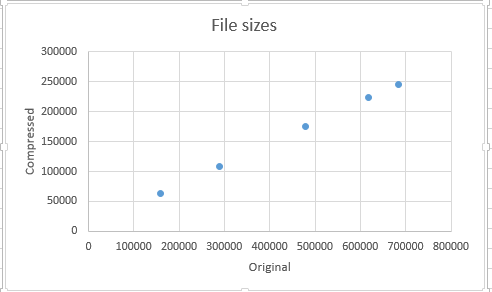
\includegraphics[width=0.5\linewidth]{file_size}
	\label{file_size}
	\caption{Scatter plot showing the compressed file size versus the original file size.}
\end{figure}

\section{Part 3}

\begin{lstlisting}
[chris@localhost opgave2]$ sleep 300&
[1] 3781
[chris@localhost opgave2]$ sleep 300&
[2] 3785
[chris@localhost opgave2]$ sleep 300&
[3] 3789
[chris@localhost opgave2]$ sleep 300&
[4] 3793
[chris@localhost opgave2]$ ps | grep "sleep"
 3781 pts/2    00:00:00 sleep
 3785 pts/2    00:00:00 sleep
 3789 pts/2    00:00:00 sleep
 3793 pts/2    00:00:00 sleep
[chris@localhost opgave2]$ 
\end{lstlisting}

\section{Part 4}

\begin{lstlisting}
[chris@localhost opgave2]$ bash S4.bash 
The surface of a rectangle with width 6 and length 7 is 42
[chris@localhost opgave2]$ 
\end{lstlisting}

\end{document}